\documentclass[12pt,letterpaper]{extarticle}
\usepackage[margin=0.58in,top=0.7in,bottom=0.67in]{geometry}
\usepackage[T1]{fontenc}
\usepackage{lmodern,tikz,fancyhdr,amsmath,amssymb}
\usetikzlibrary{arrows.meta,shapes.geometric}
\pdfinfoomitdate=1
\pdftrailerid{}
\pdfsuppressptexinfo=15
\definecolor{queueR}{RGB}{165,45,44}
\definecolor{queueB}{RGB}{34,83,151}
\pagestyle{fancy}
\fancyhf{}
\fancyhead[L]{\small Week 82 / Endless queues / Grades 3--5}
\fancyfoot[L]{\scriptsize Bellingham Math Circle / Week 82 / W82-Q-draft-v1}
\fancyfoot[R]{\scriptsize\thepage}
\renewcommand{\headrulewidth}{0.4pt}
\renewcommand{\footrulewidth}{0.4pt}
\setlength{\headheight}{16pt}
\setlength{\parindent}{0pt}
\setlength{\parskip}{8pt}
\newcommand{\problem}[2]{\textbf{Problem #1:} #2\par}
\newcommand{\card}[4]{\node[draw=#4,line width=0.85pt,rounded corners=2pt,minimum width=1.12cm,minimum height=0.95cm,fill=white,font=\normalsize] at (#1,#2) {#3};}
\newcommand{\longcard}[4]{\node[draw=#4,line width=0.85pt,rounded corners=2pt,minimum width=1.72cm,minimum height=1.05cm,fill=white,font=\large] at (#1,#2) {#3};}
\newcommand{\continuation}[4]{\draw[#4,line width=1.15pt,-{Stealth[length=2.8mm]}] (#1,#2)--++(3.4,0);\node[align=center,font=\small,text=#4] at (#1+1.7,#2-0.85) {#3};}
\newcommand{\ruleline}{\vspace{0.6cm}\hrule height0.3pt\vspace{0.6cm}\hrule height0.3pt}
\begin{document}

Queues run from left to right. A match gives each customer exactly one partner in the other queue. Nobody is left out. It keeps order when any two customers and their partners appear in the same order.

\begin{center}
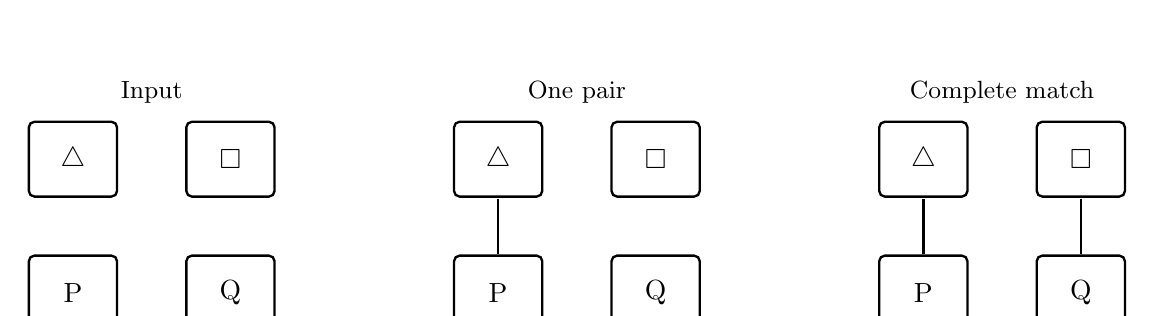
\begin{tikzpicture}[x=1cm,y=1cm]
\foreach \x/\caption in {0/Input,5.4/One pair,10.8/Complete match}{
  \node[font=\small] at (\x+1.7,0.55) {\caption};
  \card{\x+0.7}{-0.3}{$\triangle$}{black}
  \card{\x+2.7}{-0.3}{$\square$}{black}
  \card{\x+0.7}{-2.0}{P}{black}
  \card{\x+2.7}{-2.0}{Q}{black}
}
\draw[line width=0.9pt] (6.1,-0.8)--(6.1,-1.5);
\draw[line width=0.9pt] (11.5,-0.8)--(11.5,-1.5);
\draw[line width=0.9pt] (13.5,-0.8)--(13.5,-1.5);
\end{tikzpicture}
\end{center}

\problem{1}{Find every match between these two queues. Which matches keep order? Use cards and yarn to test your matches.}

\begin{center}
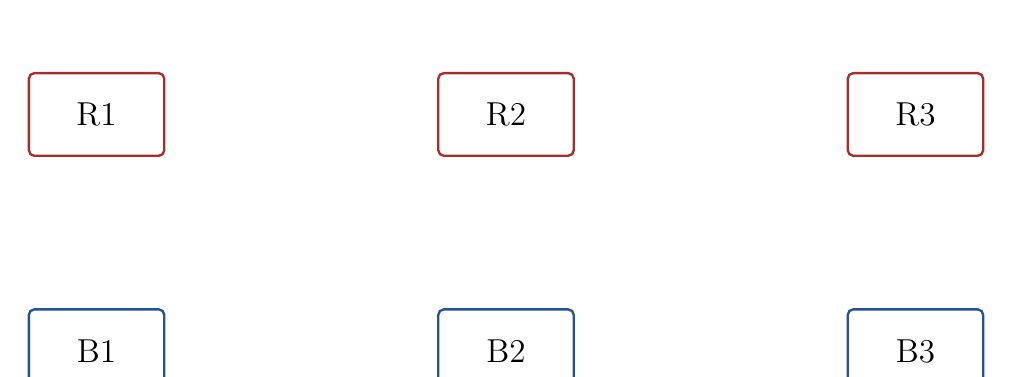
\begin{tikzpicture}[x=1cm,y=1cm]
\foreach \x/\n in {2/1,7.2/2,12.4/3}{
 \longcard{\x}{0}{R\n}{queueR}
 \longcard{\x}{-3.0}{B\n}{queueB}
}
\end{tikzpicture}
\end{center}
\vspace{0.6cm}
\ruleline
\vspace{0.8cm}
\ruleline

\newpage
An arrow marked ``numbers continue forever'' represents all later numbered customers.

\problem{2}{Compare A with B, then A with C. Can you match every customer? Can a match keep order? Give a rule for every customer, or explain why it is impossible.}

\begin{center}
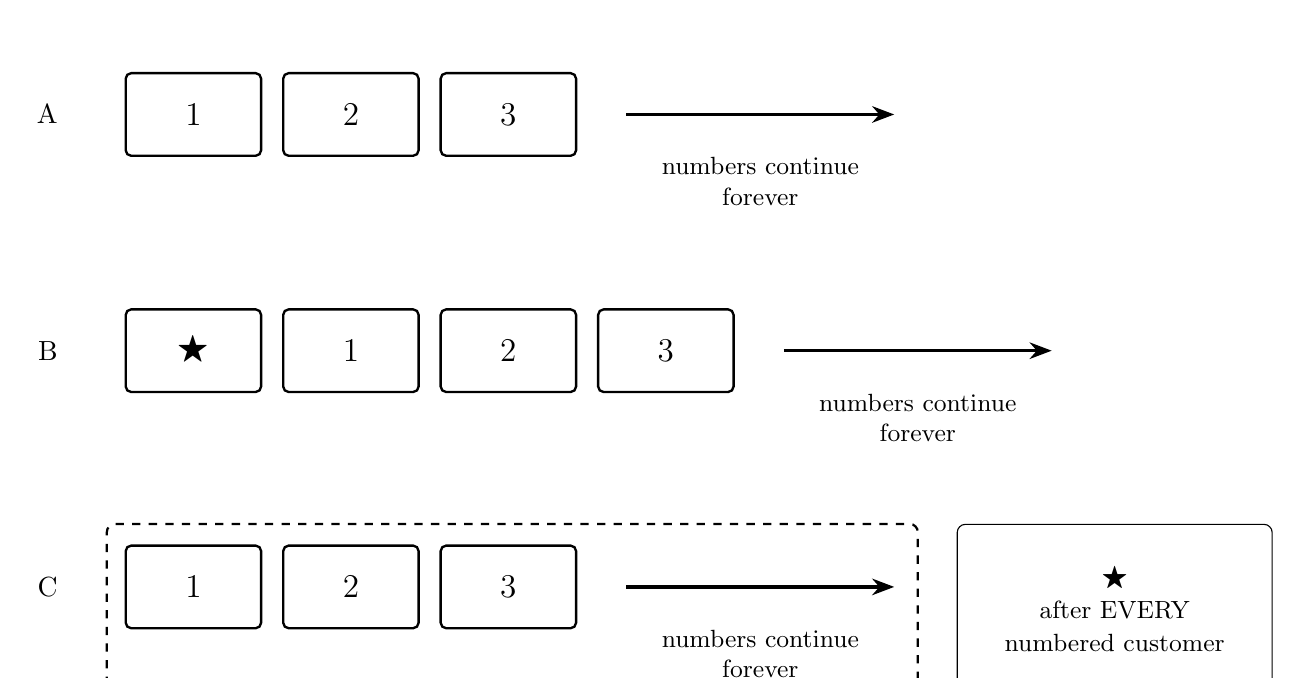
\begin{tikzpicture}[x=1cm,y=1cm]
\node[anchor=east] at (0.4,0) {A};
\foreach \x/\n in {2/1,4/2,6/3}{\longcard{\x}{0}{\n}{black}}
\continuation{7.5}{0}{numbers continue\\forever}{black}
\node[anchor=east] at (0.4,-3.0) {B};
\longcard{2}{-3.0}{$\bigstar$}{black}
\foreach \x/\n in {4/1,6/2,8/3}{\longcard{\x}{-3.0}{\n}{black}}
\continuation{9.5}{-3.0}{numbers continue\\forever}{black}
\node[anchor=east] at (0.4,-6.0) {C};
\draw[rounded corners=3pt,dashed,line width=0.8pt] (0.9,-7.35) rectangle (11.2,-5.2);
\foreach \x/\n in {2/1,4/2,6/3}{\longcard{\x}{-6.0}{\n}{black}}
\continuation{7.5}{-6.0}{numbers continue\\forever}{black}
\node[draw,rounded corners=3pt,align=center,minimum width=4.0cm,minimum height=2.15cm] at (13.7,-6.28) {$\bigstar$\\\small after EVERY\\\small numbered customer};
\end{tikzpicture}
\end{center}
\vspace{0.3cm}
\ruleline
\vspace{0.7cm}
\ruleline

\newpage
\problem{3}{Compare D with E. Can you match every customer? Can a match keep order? Give a rule for every customer, or explain why it is impossible.}

\begin{center}
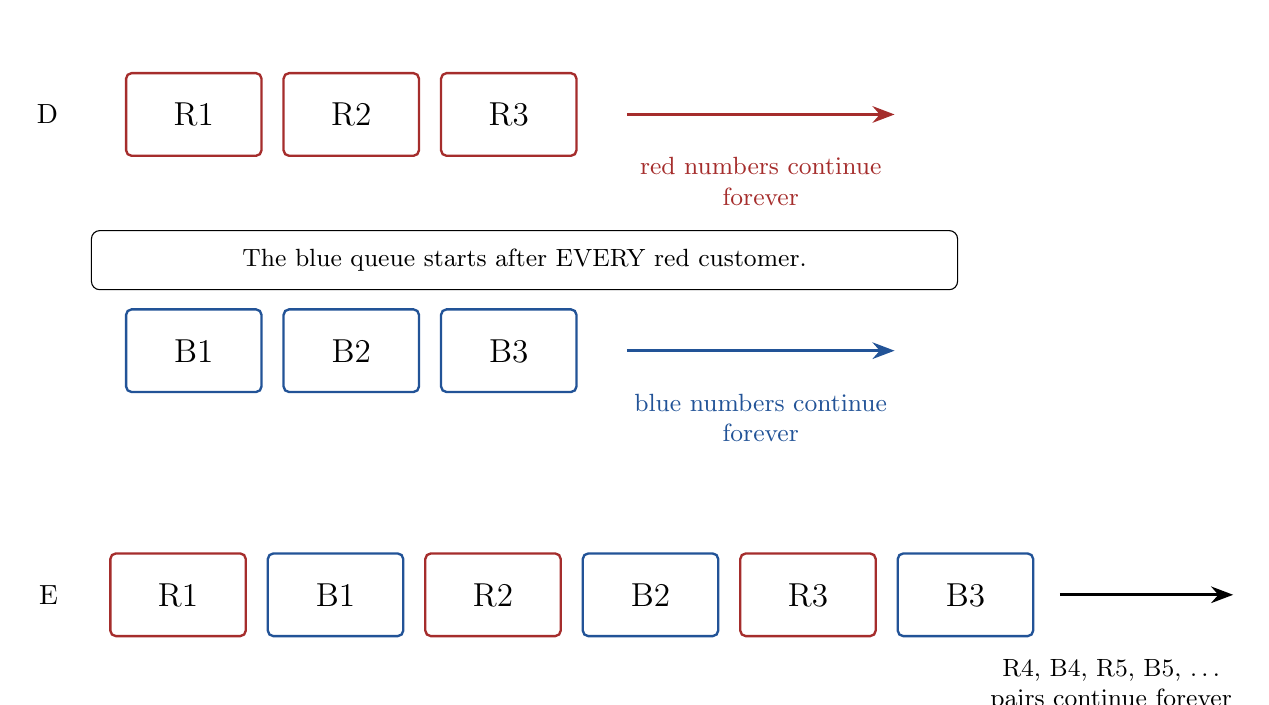
\begin{tikzpicture}[x=1cm,y=1cm]
\node[anchor=east] at (0.4,0) {D};
\foreach \x/\n in {2/1,4/2,6/3}{\longcard{\x}{0}{R\n}{queueR}}
\continuation{7.5}{0}{red numbers continue\\forever}{queueR}
\node[draw,rounded corners=3pt,align=center,minimum width=11.0cm,minimum height=0.75cm,font=\small] at (6.2,-1.85) {The blue queue starts after EVERY red customer.};
\foreach \x/\n in {2/1,4/2,6/3}{\longcard{\x}{-3.0}{B\n}{queueB}}
\continuation{7.5}{-3.0}{blue numbers continue\\forever}{queueB}
\node[anchor=east] at (0.4,-6.1) {E};
\foreach \x/\v/\c in {1.8/R1/queueR,3.8/B1/queueB,5.8/R2/queueR,7.8/B2/queueB,9.8/R3/queueR,11.8/B3/queueB}{\longcard{\x}{-6.1}{\v}{\c}}
\draw[line width=1.1pt,-{Stealth[length=2.8mm]}] (13.0,-6.1)--(15.2,-6.1);
\node[font=\small,align=center] at (13.65,-7.25) {R4, B4, R5, B5, $\ldots$\\pairs continue forever};
\end{tikzpicture}
\end{center}
\vspace{0.65cm}
\ruleline
\vspace{0.7cm}
\ruleline

\newpage
\problem{4}{Arrange one or two endless numbered rows and up to two $\bigstar$ customers on the table. A star or new row following a whole endless row comes after EVERY customer in that row.}

Find two different arrangements that can be matched while keeping order. Find two that can be matched only if order may change. Sketch your arrangements in the boxes. Give matching rules or explain the obstruction.

\begin{center}
\begin{tikzpicture}[x=1cm,y=1cm]
\foreach \y in {0,-6.3}{
 \draw[gray,rounded corners=3pt,line width=0.55pt] (0,\y) rectangle (16.1,\y-2.0);
 \draw[gray,rounded corners=3pt,line width=0.55pt] (0,\y-3.0) rectangle (16.1,\y-5.0);
}
\end{tikzpicture}
\end{center}
\vspace{0.25cm}
\ruleline

\newpage
\begin{center}
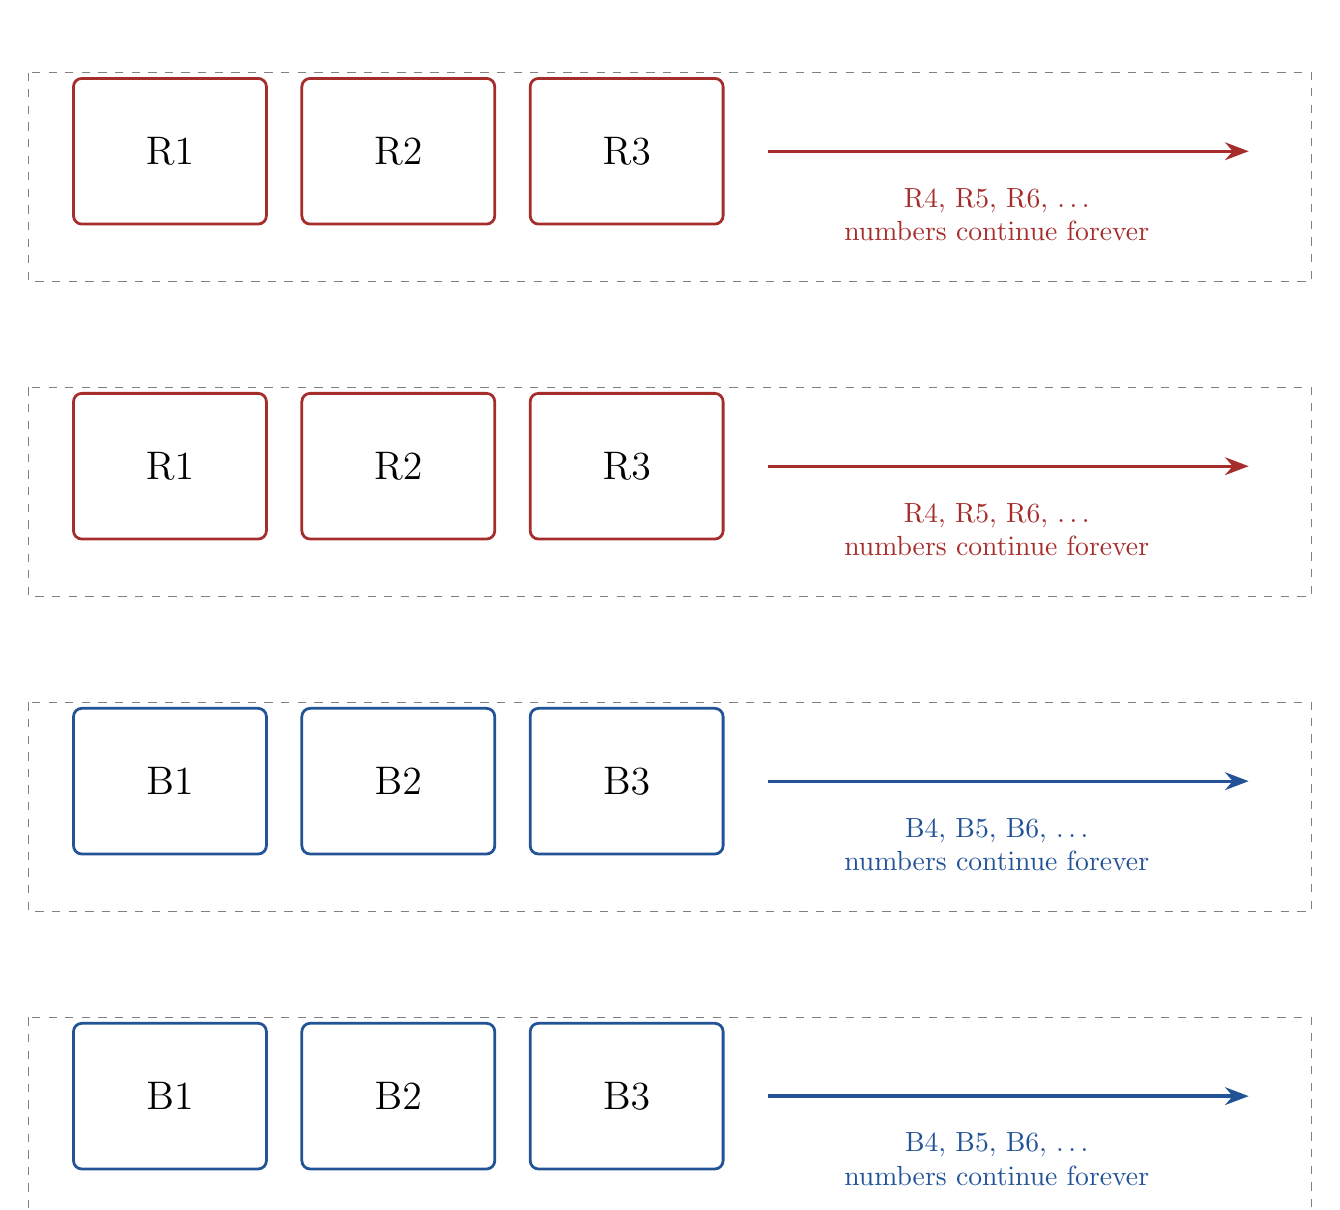
\begin{tikzpicture}[x=1cm,y=1cm]
\foreach \y/\c/\letter in {0/queueR/R,-4.0/queueR/R,-8.0/queueB/B,-12.0/queueB/B}{
 \draw[dashed,gray] (-0.3,\y+1.0) rectangle (16.0,\y-1.65);
 \foreach \x/\n in {1.5/1,4.4/2,7.3/3}{\node[draw=\c,line width=1pt,minimum width=2.45cm,minimum height=1.85cm,rounded corners=3pt,font=\Large] at (\x,\y) {\letter\n};}
 \draw[\c,line width=1.2pt,-{Stealth[length=3mm]}] (9.1,\y)--(15.2,\y);
 \node[font=\normalsize,text=\c,align=center] at (12.0,\y-0.8) {\letter4, \letter5, \letter6, $\ldots$\\numbers continue forever};
}
\end{tikzpicture}
\end{center}

\newpage
\begin{center}
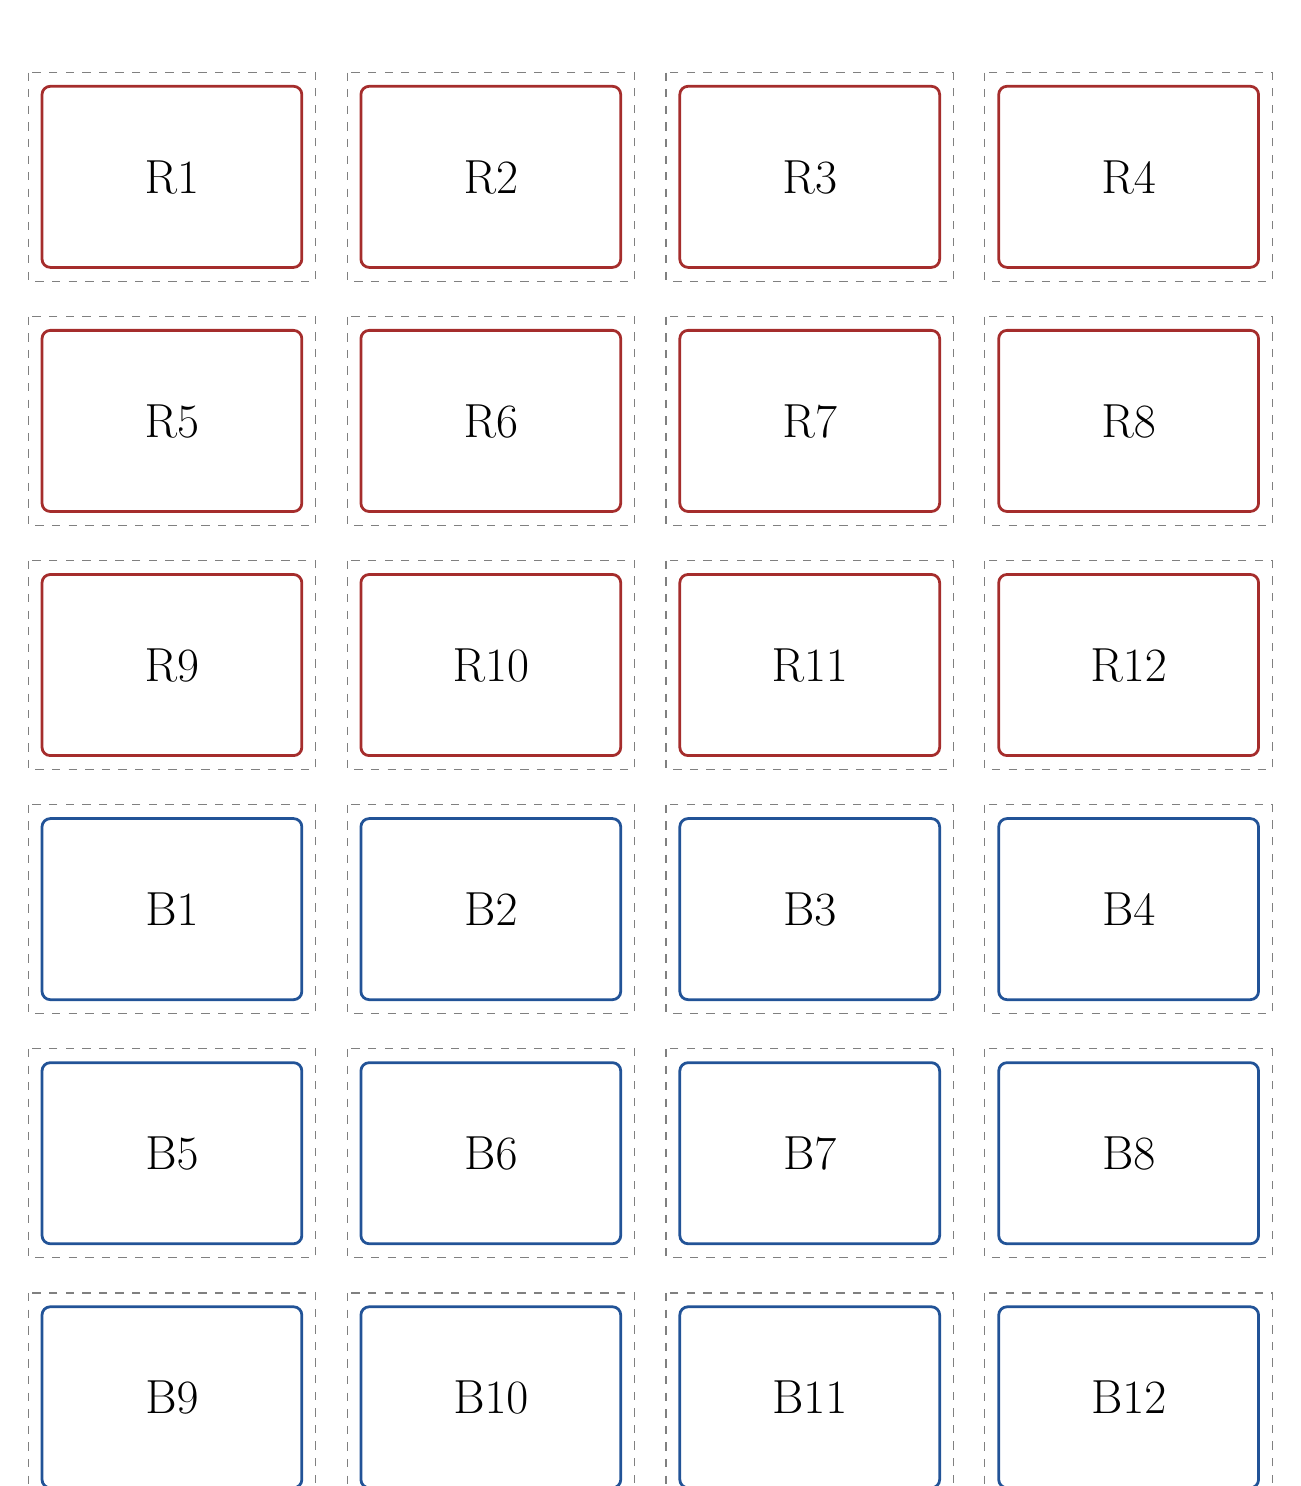
\begin{tikzpicture}[x=1cm,y=1cm]
\foreach \row/\letter/\c/\offset in {0/R/queueR/0,1/R/queueR/4,2/R/queueR/8,3/B/queueB/0,4/B/queueB/4,5/B/queueB/8}{
 \foreach \col in {0,1,2,3}{
  \pgfmathtruncatemacro{\n}{\offset+\col+1}
  \draw[dashed,gray] (4.05*\col, -3.1*\row) rectangle ++(3.65,-2.65);
  \node[draw=\c,line width=1pt,rounded corners=3pt,minimum width=3.3cm,minimum height=2.3cm,font=\LARGE] at (4.05*\col+1.825,-3.1*\row-1.325) {\letter\n};
 }
}
\end{tikzpicture}
\end{center}

\newpage
\begin{center}
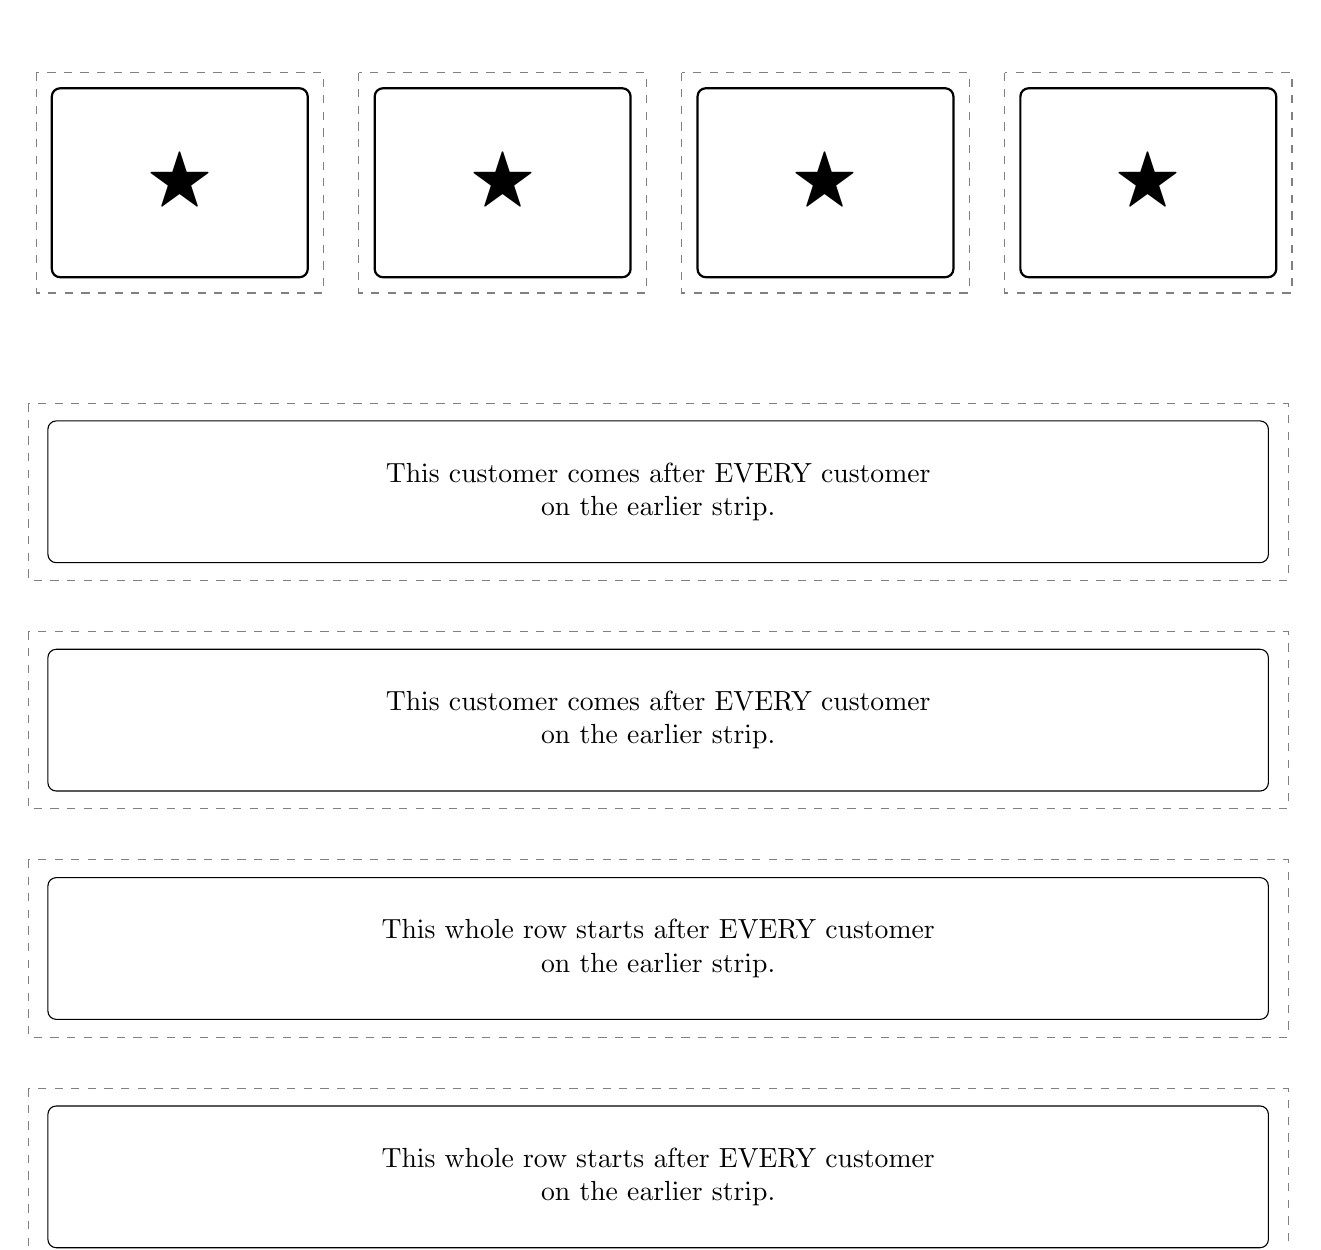
\begin{tikzpicture}[x=1cm,y=1cm]
\foreach \x in {0,4.1,8.2,12.3}{
 \draw[dashed,gray] (\x,0) rectangle ++(3.65,-2.8);
 \node[draw,line width=0.8pt,rounded corners=3pt,minimum width=3.25cm,minimum height=2.4cm,font=\Huge] at (\x+1.825,-1.4) {$\bigstar$};
}
\foreach \y in {-4.2,-7.1}{
 \draw[dashed,gray] (-0.1,\y) rectangle ++(16.0,-2.25);
 \node[draw,rounded corners=3pt,align=center,minimum width=15.5cm,minimum height=1.8cm] at (7.9,\y-1.125) {This customer comes after EVERY customer\\on the earlier strip.};
}
\foreach \y in {-10.0,-12.9}{
 \draw[dashed,gray] (-0.1,\y) rectangle ++(16.0,-2.25);
 \node[draw,rounded corners=3pt,align=center,minimum width=15.5cm,minimum height=1.8cm] at (7.9,\y-1.125) {This whole row starts after EVERY customer\\on the earlier strip.};
}
\end{tikzpicture}
\end{center}

\end{document}
